The first addition to the original drone is a small tilt gimbal
(shown in Figures \ref{figure:tilt_gimbal_base} and \ref{figure:tilt_gimbal_camera_mount}),
that is mounted on the front of the drone.
The tilt gimbal includes a mount for a standard Raspberry Pi camera module and a space for a micro servo that serves
as the gimbal's actuator.
Its rotational axis is supported by a single screw and the rotational axis of the micro servo.
The camera module is attached with screws, and its ribbon cable extends upwards above the drone body.

\begin{figure}
    \centering
    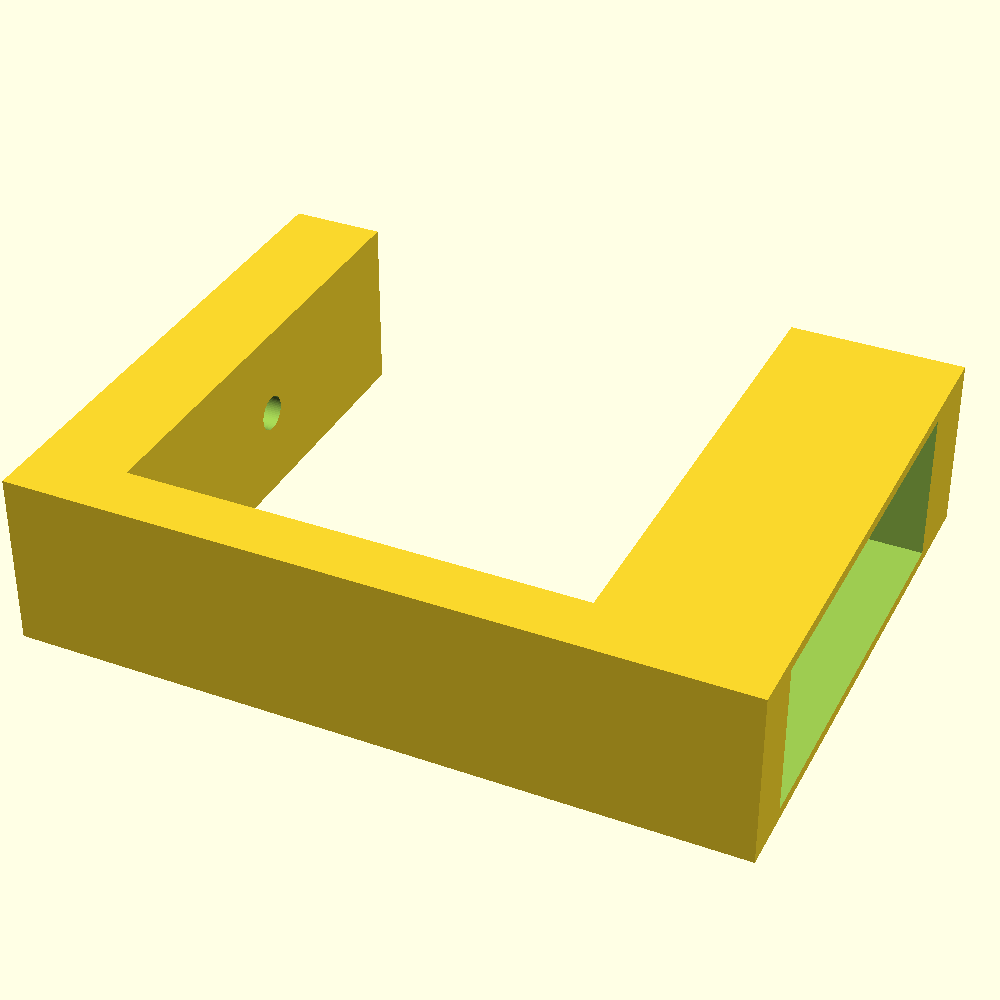
\includegraphics[width=0.75\columnwidth]{images/gimbal_base.png}
    \caption{The tilt gimbal base.}
    \label{figure:tilt_gimbal_base}
\end{figure}

\begin{figure}
    \centering
    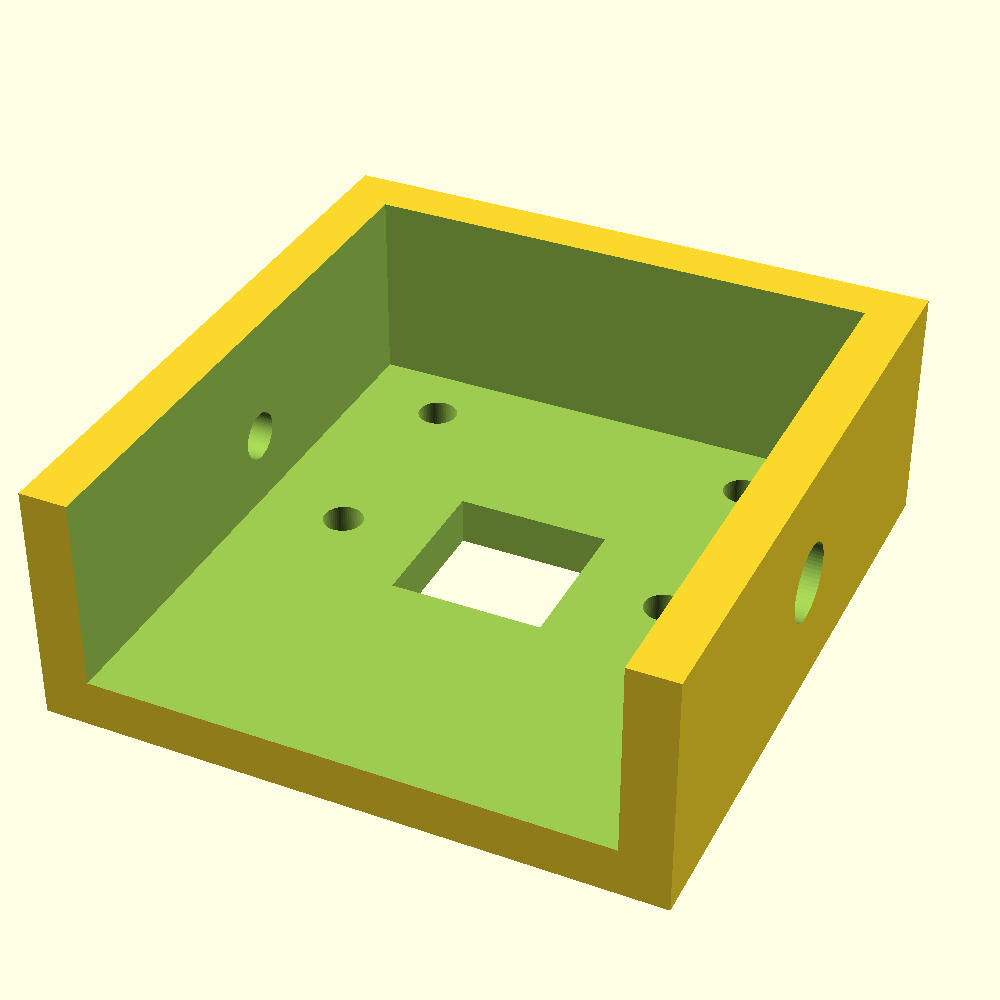
\includegraphics[width=0.75\columnwidth]{images/gimbal_camera_mount.png}
    \caption{The tilt gimbal camera mount.}
    \label{figure:tilt_gimbal_camera_mount}
\end{figure}

The second addition is a set of mounts for the drone's electronic speed controllers.
The speed controllers fit into slots on the drone's body and are held in place simply with electrical tape.